% Saberes básicos (LOMLOE) asociados a esta unidad
%
% Bloque E. El cambio
%   - Interpretación macroscópica y microscópica de las reacciones químicas: explicación de las
%     relaciones de la química con el medio ambiente, la tecnología y la sociedad.
%     Justificación: se explica el mecanismo de una reacción química (choques efectivos entre
%     partículas) y se relacionan las reacciones químicas con la tecnología, el medio ambiente y
%     la sociedad (combustión, efecto invernadero, lluvia ácida, química verde).
%   - Ley de conservación de la masa y de la ley de las proporciones definidas: aplicación de
%     estas leyes como evidencias experimentales que permiten validar el modelo atómico-molecular
%     de la materia.
%     Justificación: se introduce la ley de conservación de la masa de Lavoisier y se aplica al
%     ajuste de ecuaciones químicas y a problemas numéricos con masas de reactivos y productos.
%   - Factores que afectan a las reacciones químicas: predicción cualitativa de la evolución de
%     las reacciones, entendiendo su importancia en la resolución de problemas actuales por parte
%     de la ciencia.
%     Justificación: se estudian la temperatura, la concentración, la superficie de contacto y
%     los catalizadores como factores que modifican la velocidad de una reacción, con ejemplos
%     cotidianos e industriales (motores, conservación de alimentos, enzimas...).
%
% (Unidad separada de la antigua «Change of Matter»: los cambios físicos y químicos y la
%  separación de mezclas están en la Unidad 5, Change of Matter.)

\spacing{1.3}
\raggedbottom % pages with large figures end where the text ends (no stretched gaps between boxes)

In the previous unit we saw that in a \textbf{chemical change} new substances appear. In this unit we will study these changes in detail: how a \textbf{chemical reaction} takes place, how it is written as a \textbf{chemical equation} and why the \textbf{mass is conserved}.

\section{Chemical reactions}

\begin{definition}[Chemical reaction]
    A process in which some substances, the \textbf{reactants}, are transformed into new substances, the \textbf{products}.
\end{definition}

\subsection{How does a chemical reaction take place?}

\begin{enumerate}[label=\numberballmDarkTeal]
    \item The particles of the reactants \textbf{collide}.
    \item If they collide with enough energy and in the right direction (an \textbf{effective collision}), the bonds between their atoms break.
    \item The atoms \textbf{rearrange} and form new molecules: the products.
\end{enumerate}

\begin{figure}[H]
    \centering
    % [FIGURA ORIGINAL] \includegraphics[width=\textwidth]{Unit_6/collisions}
    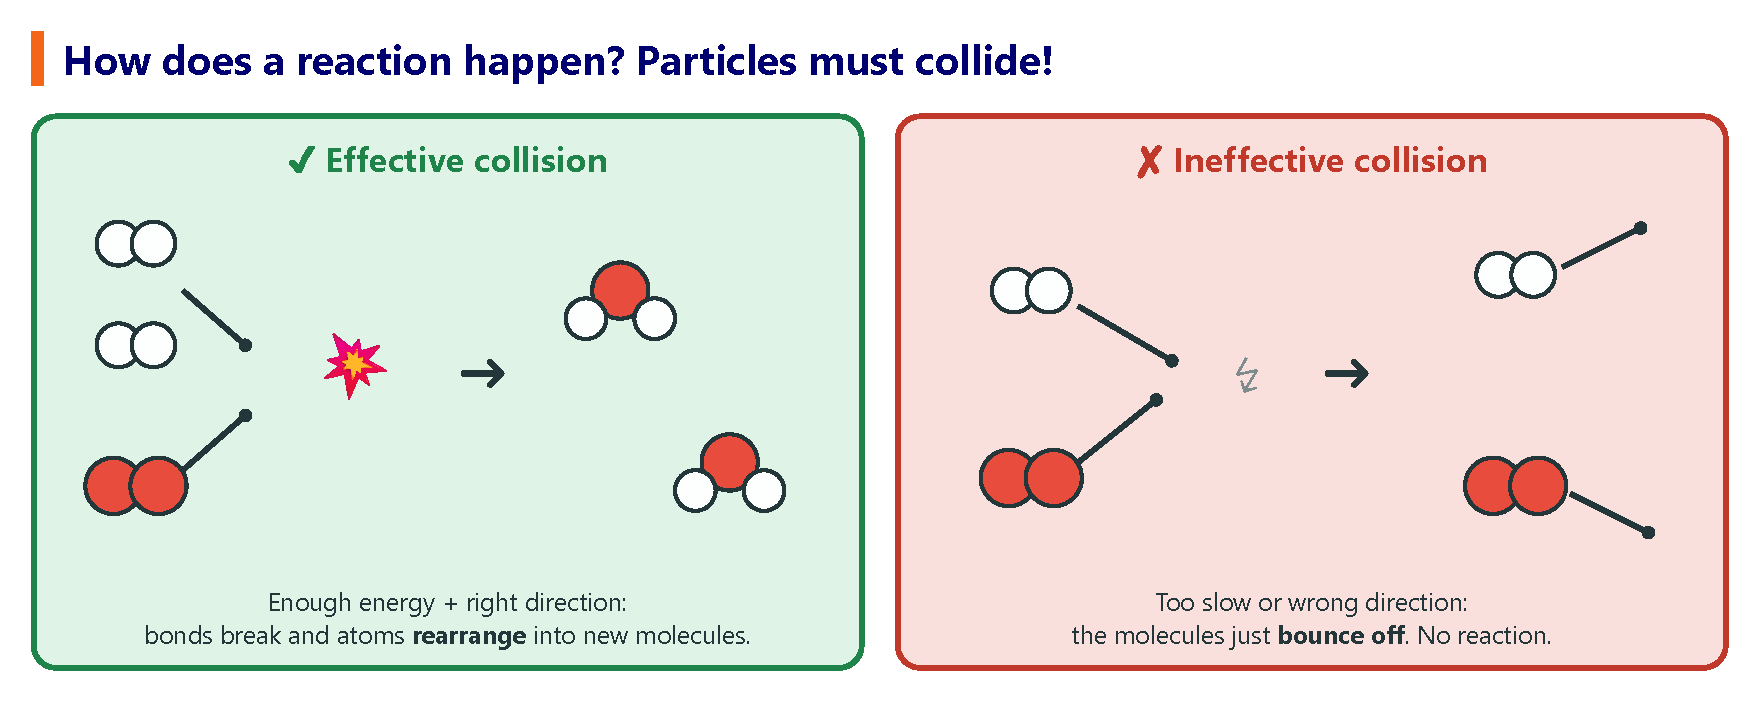
\includegraphics[width=\textwidth]{FigurasSVG/Unit_6_Chemical_Reactions/pdf/collisions.pdf}
    \caption{Only effective collisions produce a reaction: \(2\ch{H2} + \ch{O2} \longrightarrow 2\ch{H2O}\).}
    \label{fig:u6_collisions}
\end{figure}

\begin{exercise}
    Hydrogen and oxygen molecules are inside a container. In collision A, the molecules hit each other very gently; in collision B, they hit each other fast and head-on. In which case is a reaction more likely? Why?
    \begin{solu}
        In \textbf{collision B}. An effective collision needs \textbf{enough energy} and the right orientation. In collision A the molecules hit too gently, so their bonds do not break and they simply bounce off.
    \end{solu}
\end{exercise}

\begin{exercise}
    Hydrogen peroxide (\ch{H2O2}) can be formed from hydrogen (\ch{H2}) and oxygen (\ch{O2}).
    \begin{enumerate}[label=\letraminuscula]
        \item Identify the reactants and the products.
        \item Which are simple substances and which is a compound?
    \end{enumerate}
    \begin{solu}
        \begin{enumerate}[label=\alph*)]
            \item Reactants: \ch{H2} and \ch{O2}. Product: \ch{H2O2}.
            \item \ch{H2} and \ch{O2} are \textbf{simple substances}; \ch{H2O2} is a \textbf{compound}.
        \end{enumerate}
    \end{solu}
\end{exercise}

\begin{exercise}
    True or false? Correct the false statements.
    \begin{enumerate}[label=\letraminuscula]
        \item Every collision between reactant particles produces a chemical reaction.
        \item An effective collision needs enough energy and the correct orientation.
        \item Products are formed when the bonds of the reactants break and the atoms rearrange.
    \end{enumerate}
    \begin{solu}
        \begin{enumerate}[label=\alph*)]
            \item \textbf{False}: only \textit{effective} collisions produce a reaction.
            \item \textbf{True}.
            \item \textbf{True}.
        \end{enumerate}
    \end{solu}
\end{exercise}

\subsection{Chemical equations and the law of conservation of mass}

\begin{definition}[Chemical equation]
    The way we write a reaction with chemical formulas: reactants on the left, products on the right, and an arrow between them.
    \begin{equation*}
        \underbrace{\ch{N2} + 3\ch{H2}}_{\text{reactants}} \longrightarrow \underbrace{2\ch{NH3}}_{\text{products}}
    \end{equation*}
\end{definition}

\begin{figure}[H]
    \centering
    % [FIGURA ORIGINAL] \includegraphics[width=\textwidth]{Unit_6/conservation_mass}
    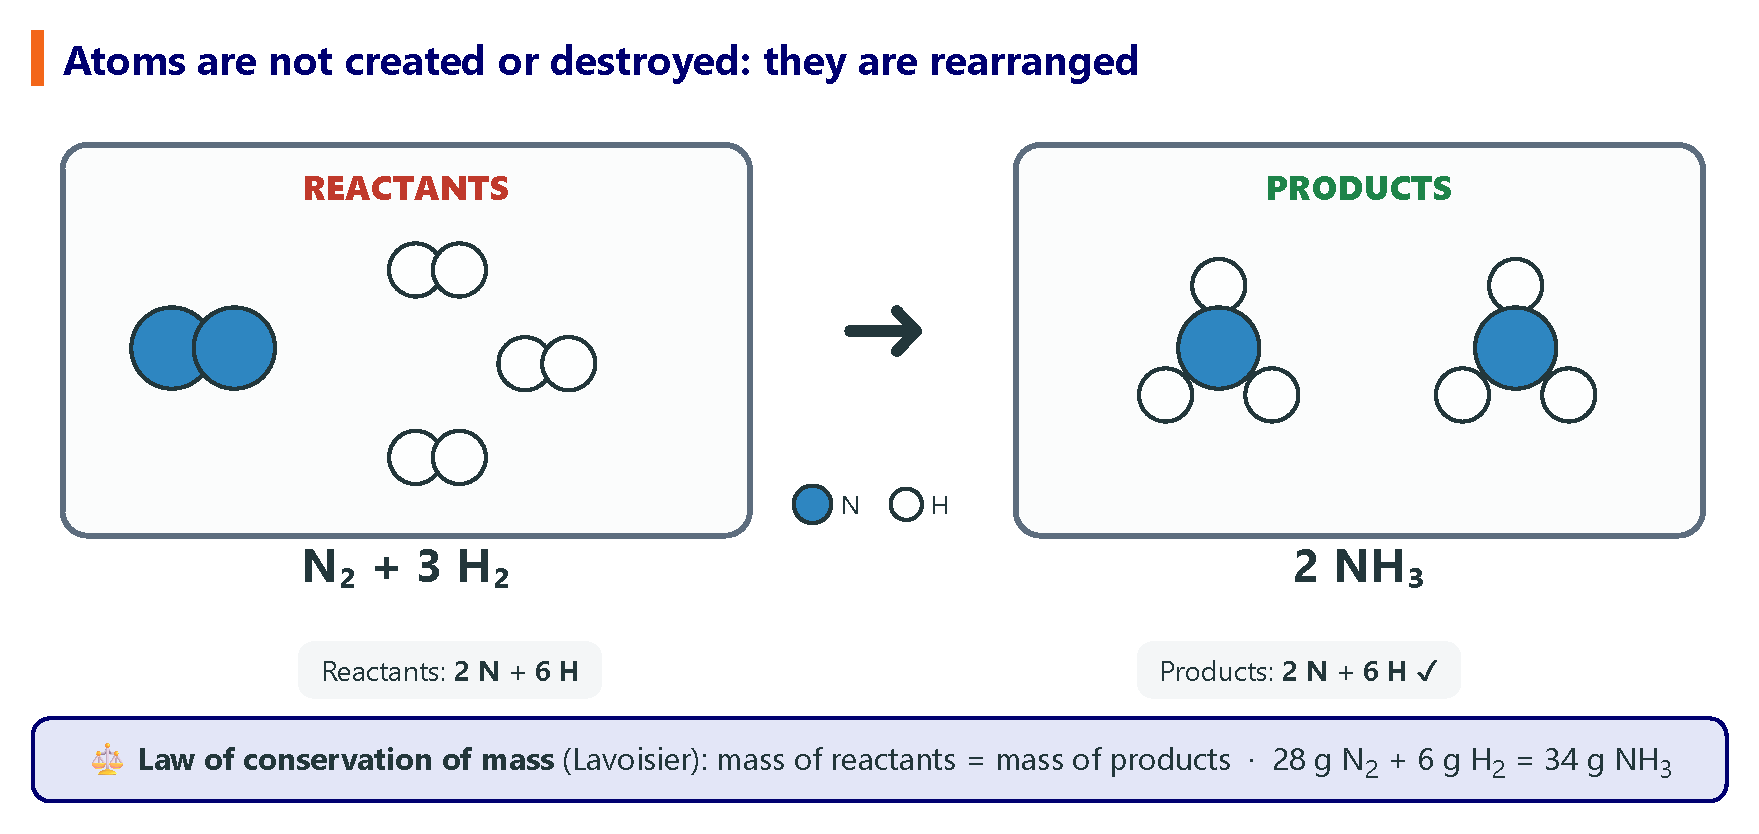
\includegraphics[width=\textwidth]{FigurasSVG/Unit_6_Chemical_Reactions/pdf/conservation_mass.pdf}
    \caption{The same atoms before and after: only the way they are joined changes.}
    \label{fig:u6_conservation_mass}
\end{figure}

\begin{definition}[Law of conservation of mass]
    In a chemical reaction, the total mass of the reactants is \textbf{equal} to the total mass of the products. Matter is not created or destroyed, only transformed (Lavoisier, 18th century).
\end{definition}

\begin{didyouknow}
    Antoine Lavoisier, the ``father of modern chemistry'', weighed everything very carefully in closed containers, which is how he discovered the law of conservation of mass. His famous sentence was: ``\emph{Nothing is lost, nothing is created, everything is transformed}''.
\end{didyouknow}

\begin{example}
    \textbf{Worked example: using the law of conservation of mass step by step.} When limestone (calcium carbonate, \ch{CaCO3}) is heated strongly, it decomposes into quicklime (calcium oxide, \ch{CaO}) and carbon dioxide gas (\ch{CO2}). We heat \qty{50}{\g} of calcium carbonate in a closed container until it has all reacted, and we obtain \qty{28}{\g} of calcium oxide. What mass of carbon dioxide has been formed?
    \begin{enumerate}[label=\numberballmDarkTeal]
        \item \textbf{Identify the reactants and the products.} The reactant is calcium carbonate; the products are calcium oxide and carbon dioxide:
        \[
            \ch{CaCO3} \longrightarrow \ch{CaO} + \ch{CO2}
        \]
        \item \textbf{Write down the data and the unknown.} \(m(\ch{CaCO3}) = \qty{50}{\g}\); \quad \(m(\ch{CaO}) = \qty{28}{\g}\); \quad \(m(\ch{CO2}) = \ ?\)
        \item \textbf{Apply the law of conservation of mass.} The total mass of the reactants is equal to the total mass of the products:
        \[
            m(\ch{CaCO3}) = m(\ch{CaO}) + m(\ch{CO2})
        \]
        \item \textbf{Substitute the data.}
        \[
            \qty{50}{\g} = \qty{28}{\g} + m(\ch{CO2})
        \]
        \item \textbf{Isolate the unknown.} The \qty{28}{\g} that are adding on the right go to the left subtracting:
        \[
            m(\ch{CO2}) = \qty{50}{\g} - \qty{28}{\g} = \textcolor{red}{\qty{22}{\g}}
        \]
        \item \textbf{Check the result.} Reactants: \qty{50}{\g}. Products: \(\qty{28}{\g} + \qty{22}{\g} = \qty{50}{\g}\). The masses are equal, so the answer is correct.
    \end{enumerate}
    \textbf{Why a closed container?} If we heat the limestone in an open container, the \ch{CO2} escapes into the air and the balance shows only \qty{28}{\g} at the end: it \emph{seems} that \qty{22}{\g} have been lost. The mass has not disappeared; it has simply left as a gas. That is why Lavoisier always weighed his reactions in closed containers.
\end{example}

\begin{exercise}
    \qty{4}{\g} of hydrogen react completely with \qty{32}{\g} of oxygen, forming water. What mass of water is obtained?
    \begin{solu}
        \(m(\ch{H2O}) = m(\ch{H2}) + m(\ch{O2}) = \qty{4}{\g} + \qty{32}{\g} = \qty{36}{\g}\).
    \end{solu}
\end{exercise}

\begin{exercise}
    \qty{5.6}{\g} of iron react completely with sulphur, giving \qty{8.8}{\g} of iron sulphide (\ch{FeS}). What mass of sulphur reacted?
    \begin{solu}
        \(m(\ch{S}) = m(\ch{FeS}) - m(\ch{Fe}) = \qty{8.8}{\g} - \qty{5.6}{\g} = \qty{3.2}{\g}\).
    \end{solu}
\end{exercise}

\begin{exercise}
    \qty{16}{\g} of methane (\ch{CH4}) burn completely with \qty{64}{\g} of oxygen, producing \qty{44}{\g} of carbon dioxide and some water vapour. What mass of water vapour is produced?
    \begin{solu}
        \(m(\ch{CH4}) + m(\ch{O2}) = m(\ch{CO2}) + m(\ch{H2O})\) \\
        \(\qty{16}{\g} + \qty{64}{\g} = \qty{44}{\g} + m(\ch{H2O}) \;\to\; m(\ch{H2O}) = \qty{36}{\g}\).
    \end{solu}
\end{exercise}

\subsection{Balancing chemical equations}

% Marks for the balancing tables: element balanced / not balanced
\providecommand{\balok}{\textcolor{green!50!black}{\(\checkmark\)}}
\providecommand{\balno}{\textcolor{red}{\(\boldsymbol{\times}\)}}

Balancing a chemical equation is one of the most important skills in chemistry. Atoms are not created or destroyed in a reaction (law of conservation of mass), so the equation must show \textbf{the same atoms} before and after the reaction.

\begin{definition}[Balanced chemical equation]
    A chemical equation that has the \textbf{same number of atoms of each element} on the reactants side (left) and on the products side (right).
\end{definition}

\begin{impt}
    \negsubro{The three basic rules}
    \begin{enumerate}[label=\numberballmDarkTeal]
        \item In the \textbf{reactants} there must be the \textbf{same number of atoms of each element} as in the \textbf{products}.
        \item We \textbf{count} the atoms of each element, one element at a time, in the reactants (\textbf{left}) and in the products (\textbf{right}).
        \item To make it easier, it is \textbf{advisable} to leave \textbf{hydrogen} and \textbf{oxygen} until the \textbf{end}, and oxygen the very last.
    \end{enumerate}
\end{impt}

\subsubsection{Stoichiometric coefficients}

To balance an equation we can only write numbers \textbf{in front of} the formulas. These numbers are called \negsubro{stoichiometric coefficients}.

\begin{definition}[Stoichiometric coefficient]
    A whole number (1, 2, 3\ldots) written \textbf{in front of} a formula in a chemical equation. It \textbf{multiplies} all the atoms of that formula. A coefficient of 1 is not written.
\end{definition}

\begin{figure}[H]
    \centering
    % [FIGURA ORIGINAL] \includegraphics[width=\textwidth]{Unit_6/coefficient_subscript}
    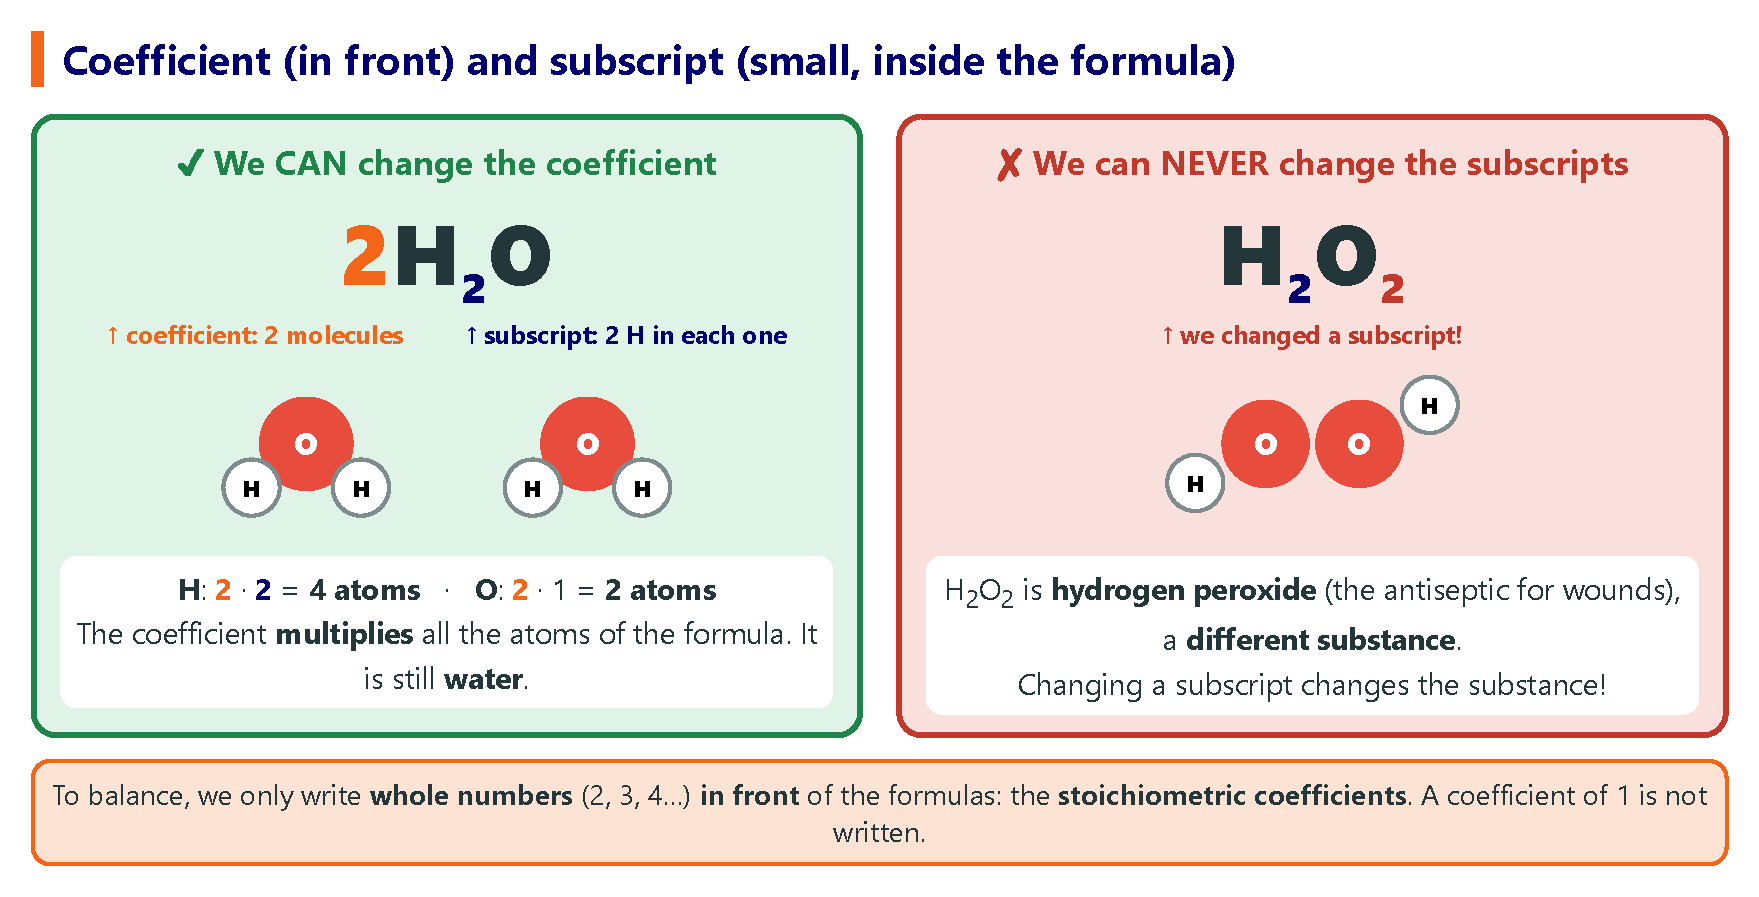
\includegraphics[width=\textwidth]{FigurasSVG/Unit_6_Chemical_Reactions/pdf/coefficient_subscript.pdf}
    \caption{The coefficient multiplies the whole formula; the subscripts can never be changed.}
    \label{fig:u6_coefficient_subscript}
\end{figure}

\begin{marker}
    \begin{itemize}
        \item The coefficients are written \textbf{in front} of the formula and \textbf{NEVER as a subscript}. If we change a subscript, we change the substance: \ch{H2O} is water, but \ch{H2O2} is hydrogen peroxide.
        \item Once we write a coefficient, it \textbf{multiplies the subscripts} of all the elements of that formula, so the number of atoms of \textbf{every} element in the formula changes: in \(3\ch{CO2}\) there are \(3 \cdot 1 = 3\) C and \(3 \cdot 2 = 6\) O.
        \item The coefficients must always be \textbf{whole numbers}: 1, 2, 3\ldots{} (never 1,5 or \(\frac{1}{2}\)).
    \end{itemize}
\end{marker}

\subsubsection{The method, step by step}

\begin{enumerate}[label=\numberballmDarkTeal]
    \item Write the equation and, \textbf{below it, a table}: one row for each element, and under each formula the number of atoms of that element. Add a column with the total on the left and another with the total on the right.
    \item Take the elements one by one: first the metals and the other elements, then \textbf{hydrogen} and finally \textbf{oxygen}.
    \item For each element, compare the total on the left with the total on the right:
    \begin{itemize}
        \item If they are \textbf{the same}, the element is balanced. We \textbf{keep} the coefficients and go on to the next element.
        \item If they are \textbf{different}, we go to the side with \textbf{fewer} atoms of that element and write in front of the formula that contains it a coefficient \textbf{one unit bigger} (if there is no number, it is a 1, so we write a 2). We \textbf{count again}. If the two sides are still different, we again increase by one the coefficient on the side that \textbf{now} has fewer atoms, and repeat until both sides are equal.
    \end{itemize}
    \item \textbf{Be careful}: when we write a coefficient, we also change the other elements of that formula. So, every time we balance a new element, we must \textbf{check again} that the elements we had already balanced are still balanced. If one is not, we balance it again.
    \item When \textbf{all} the elements are balanced, the equation is balanced. If all the coefficients can be divided by the same number, we simplify them (\(2, 4, 2 \to 1, 2, 1\)).
\end{enumerate}

\begin{figure}[H]
    \centering
    % [FIGURA ORIGINAL] \includegraphics[width=0.95\textwidth]{Unit_6/balancing_method}
    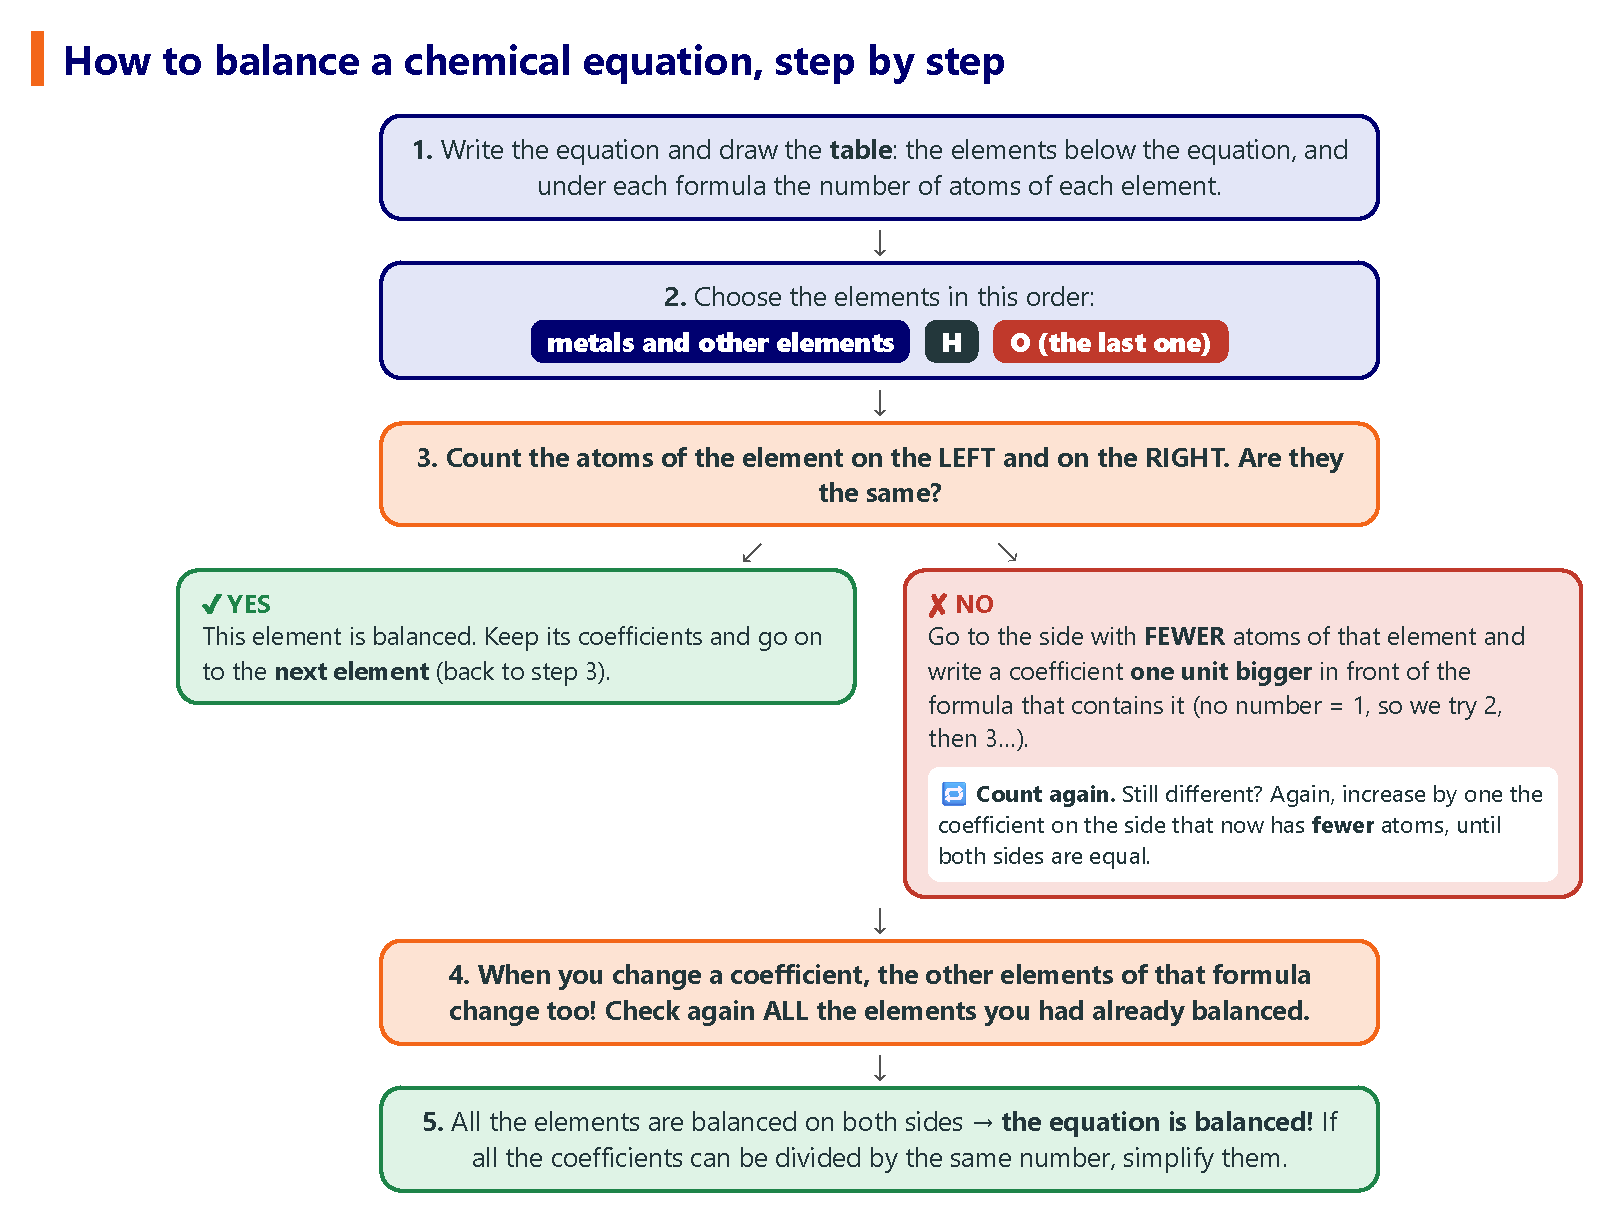
\includegraphics[width=0.95\textwidth]{FigurasSVG/Unit_6_Chemical_Reactions/pdf/balancing_method.pdf}
    \caption{The method for balancing a chemical equation.}
    \label{fig:u6_balancing_method}
\end{figure}

\begin{impt}
    \negsubro{The balancing table}: below the equation we write the elements, and under each formula the number of atoms of each element. When a formula has a coefficient, we multiply: coefficient \(\cdot\) subscript. The columns \textbf{Left} and \textbf{Right} show the totals, and the last column tells us whether that element is balanced (\balok) or not (\balno). The row of the element we are working on is \colorbox{yellow!25}{highlighted}, and the coefficient we have just written is in \textcolor{red}{\textbf{red}}.
\end{impt}

\begin{example}
    \textbf{Balance the equation for the formation of ammonia: } \(\ch{N2} + \ch{H2} \longrightarrow \ch{NH3}\)
\end{example}

\negsubro{Step 1}: we draw the table and count the atoms of each element.
\begin{center}
    \small\renewcommand{\arraystretch}{1.3}
    % --- tabla antigua ---
    % \begin{tabular}{l|cc|>{\columncolor{blue!8}}c||c|>{\columncolor{blue!8}}c|c}
        % \textbf{Element} & \ch{N2} & \ch{H2} & \textbf{Left} & \ch{NH3} & \textbf{Right} &  \\
        % \hline
        % \textbf{N} & 2 & -- & \textbf{2} & 1 & \textbf{1} & \balno \\
        % \textbf{H} & -- & 2 & \textbf{2} & 3 & \textbf{3} & \balno \\
    % \end{tabular}
    % --- tabla nueva ---
    \begin{tabular}{@{}lcccccc@{}}
        \toprule
        \textbf{Element} & \textbf{\ch{N2}} & \textbf{\ch{H2}} & \textbf{Left} & \textbf{\ch{NH3}} & \textbf{Right} &  \\
        \midrule
        \textbf{N} & 2 & -- & \textbf{2} & 1 & \textbf{1} & \balno \\[3pt]
        \textbf{H} & -- & 2 & \textbf{2} & 3 & \textbf{3} & \balno \\
        \bottomrule
    \end{tabular}
\end{center}

\negsubro{Step 2: nitrogen.} On the left there are 2 N and on the right only 1 N. The \textbf{right} side has fewer, so we write a \textbf{2} in front of \ch{NH3}. Now we count again: \(2 \cdot 1 = 2\) N on the right. \balok{} Notice that the H on the right have also changed: \(2 \cdot 3 = 6\).
\begin{center}
    \small\renewcommand{\arraystretch}{1.3}
    % --- tabla antigua ---
    % \begin{tabular}{l|cc|>{\columncolor{blue!8}}c||c|>{\columncolor{blue!8}}c|c}
        % \textbf{Element} & \ch{N2} & \ch{H2} & \textbf{Left} & \textcolor{red}{\textbf{2}}\ch{NH3} & \textbf{Right} &  \\
        % \hline
        % \rowcolor{yellow!25} \textbf{N} & 2 & -- & \textbf{2} & \(2 \cdot 1 = 2\) & \textbf{2} & \balok \\
        % \textbf{H} & -- & 2 & \textbf{2} & \(2 \cdot 3 = 6\) & \textbf{6} & \balno \\
    % \end{tabular}
    % --- tabla nueva ---
    \begin{tabular}{@{}lcccccc@{}}
        \toprule
        \textbf{Element} & \textbf{\ch{N2}} & \textbf{\ch{H2}} & \textbf{Left} & \textcolor{red}{\textbf{2}}\ch{NH3} & \textbf{Right} &  \\
        \midrule
        \textbf{N} & 2 & -- & \textbf{2} & \(2 \cdot 1 = 2\) & \textbf{2} & \balok \\[3pt]
        \textbf{H} & -- & 2 & \textbf{2} & \(2 \cdot 3 = 6\) & \textbf{6} & \balno \\
        \bottomrule
    \end{tabular}
\end{center}
\negsubro{Step 3: hydrogen.} On the left there are 2 H and on the right 6 H. The \textbf{left} side has fewer, so we increase the coefficient of \ch{H2} one unit at a time: with a 2 we get \(2 \cdot 2 = 4\) H \balno; with a 3 we get \(3 \cdot 2 = 6\) H \balok.
\begin{center}
    \small\renewcommand{\arraystretch}{1.3}
    % --- tabla antigua ---
    % \begin{tabular}{l|cc|>{\columncolor{blue!8}}c||c|>{\columncolor{blue!8}}c|c}
        % \textbf{Element} & \ch{N2} & \textcolor{red}{\textbf{3}}\ch{H2} & \textbf{Left} & 2\ch{NH3} & \textbf{Right} &  \\
        % \hline
        % \textbf{N} & 2 & -- & \textbf{2} & \(2 \cdot 1 = 2\) & \textbf{2} & \balok \\
        % \rowcolor{yellow!25} \textbf{H} & -- & \(3 \cdot 2 = 6\) & \textbf{6} & \(2 \cdot 3 = 6\) & \textbf{6} & \balok \\
    % \end{tabular}
    % --- tabla nueva ---
    \begin{tabular}{@{}lcccccc@{}}
        \toprule
        \textbf{Element} & \textbf{\ch{N2}} & \textcolor{red}{\textbf{3}}\ch{H2} & \textbf{Left} & \textbf{2\ch{NH3}} & \textbf{Right} &  \\
        \midrule
        \textbf{N} & 2 & -- & \textbf{2} & \(2 \cdot 1 = 2\) & \textbf{2} & \balok \\[3pt]
        \textbf{H} & -- & \(3 \cdot 2 = 6\) & \textbf{6} & \(2 \cdot 3 = 6\) & \textbf{6} & \balok \\
        \bottomrule
    \end{tabular}
\end{center}
\negsubro{Step 4: check.} The nitrogen is still balanced (2 = 2) and the hydrogen too (6 = 6). The balanced equation is:
\begin{equation*}
    \ch{N2} + 3\ch{H2} \longrightarrow 2\ch{NH3}
\end{equation*}

\begin{example}
    \textbf{Balance the combustion of methane (natural gas): } \(\ch{CH4} + \ch{O2} \longrightarrow \ch{CO2} + \ch{H2O}\)
\end{example}

\negsubro{Step 1}: the table. We will leave H and O for the end, and O the very last.
\begin{center}
    \small\renewcommand{\arraystretch}{1.3}
    % --- tabla antigua ---
    % \begin{tabular}{l|cc|>{\columncolor{blue!8}}c||cc|>{\columncolor{blue!8}}c|c}
        % \textbf{Element} & \ch{CH4} & \ch{O2} & \textbf{Left} & \ch{CO2} & \ch{H2O} & \textbf{Right} &  \\
        % \hline
        % \textbf{C} & 1 & -- & \textbf{1} & 1 & -- & \textbf{1} & \balok \\
        % \textbf{H} & 4 & -- & \textbf{4} & -- & 2 & \textbf{2} & \balno \\
        % \textbf{O} & -- & 2 & \textbf{2} & 2 & 1 & \textbf{3} & \balno \\
    % \end{tabular}
    % --- tabla nueva ---
    \begin{tabular}{@{}lccccccc@{}}
        \toprule
        \textbf{Element} & \textbf{\ch{CH4}} & \textbf{\ch{O2}} & \textbf{Left} & \textbf{\ch{CO2}} & \textbf{\ch{H2O}} & \textbf{Right} &  \\
        \midrule
        \textbf{C} & 1 & -- & \textbf{1} & 1 & -- & \textbf{1} & \balok \\[3pt]
        \textbf{H} & 4 & -- & \textbf{4} & -- & 2 & \textbf{2} & \balno \\[3pt]
        \textbf{O} & -- & 2 & \textbf{2} & 2 & 1 & \textbf{3} & \balno \\
        \bottomrule
    \end{tabular}
\end{center}

\negsubro{Step 2: carbon.} 1 C on the left and 1 C on the right. \balok{} We go on to the next element.

\negsubro{Step 3: hydrogen.} 4 H on the left and 2 H on the right. The \textbf{right} side has fewer, so we write a \textbf{2} in front of \ch{H2O}: \(2 \cdot 2 = 4\) H. \balok
\begin{center}
    \small\renewcommand{\arraystretch}{1.3}
    % --- tabla antigua ---
    % \begin{tabular}{l|cc|>{\columncolor{blue!8}}c||cc|>{\columncolor{blue!8}}c|c}
        % \textbf{Element} & \ch{CH4} & \ch{O2} & \textbf{Left} & \ch{CO2} & \textcolor{red}{\textbf{2}}\ch{H2O} & \textbf{Right} &  \\
        % \hline
        % \textbf{C} & 1 & -- & \textbf{1} & 1 & -- & \textbf{1} & \balok \\
        % \rowcolor{yellow!25} \textbf{H} & 4 & -- & \textbf{4} & -- & \(2 \cdot 2 = 4\) & \textbf{4} & \balok \\
        % \textbf{O} & -- & 2 & \textbf{2} & 2 & \(2 \cdot 1 = 2\) & \textbf{4} & \balno \\
    % \end{tabular}
    % --- tabla nueva ---
    \begin{tabular}{@{}lccccccc@{}}
        \toprule
        \textbf{Element} & \textbf{\ch{CH4}} & \textbf{\ch{O2}} & \textbf{Left} & \textbf{\ch{CO2}} & \textcolor{red}{\textbf{2}}\ch{H2O} & \textbf{Right} &  \\
        \midrule
        \textbf{C} & 1 & -- & \textbf{1} & 1 & -- & \textbf{1} & \balok \\[3pt]
        \textbf{H} & 4 & -- & \textbf{4} & -- & \(2 \cdot 2 = 4\) & \textbf{4} & \balok \\[3pt]
        \textbf{O} & -- & 2 & \textbf{2} & 2 & \(2 \cdot 1 = 2\) & \textbf{4} & \balno \\
        \bottomrule
    \end{tabular}
\end{center}
\negsubro{Step 4: oxygen (the last one).} On the left there are 2 O; on the right, \(2 + 2 = 4\) O (2 in \ch{CO2} and 2 in \(2\ch{H2O}\)). The \textbf{left} side has fewer, so we write a \textbf{2} in front of \ch{O2}: \(2 \cdot 2 = 4\) O. \balok
\begin{center}
    \small\renewcommand{\arraystretch}{1.3}
    % --- tabla antigua ---
    % \begin{tabular}{l|cc|>{\columncolor{blue!8}}c||cc|>{\columncolor{blue!8}}c|c}
        % \textbf{Element} & \ch{CH4} & \textcolor{red}{\textbf{2}}\ch{O2} & \textbf{Left} & \ch{CO2} & 2\ch{H2O} & \textbf{Right} &  \\
        % \hline
        % \textbf{C} & 1 & -- & \textbf{1} & 1 & -- & \textbf{1} & \balok \\
        % \textbf{H} & 4 & -- & \textbf{4} & -- & \(2 \cdot 2 = 4\) & \textbf{4} & \balok \\
        % \rowcolor{yellow!25} \textbf{O} & -- & \(2 \cdot 2 = 4\) & \textbf{4} & 2 & \(2 \cdot 1 = 2\) & \textbf{4} & \balok \\
    % \end{tabular}
    % --- tabla nueva ---
    \begin{tabular}{@{}lccccccc@{}}
        \toprule
        \textbf{Element} & \textbf{\ch{CH4}} & \textcolor{red}{\textbf{2}}\ch{O2} & \textbf{Left} & \textbf{\ch{CO2}} & \textbf{2\ch{H2O}} & \textbf{Right} &  \\
        \midrule
        \textbf{C} & 1 & -- & \textbf{1} & 1 & -- & \textbf{1} & \balok \\[3pt]
        \textbf{H} & 4 & -- & \textbf{4} & -- & \(2 \cdot 2 = 4\) & \textbf{4} & \balok \\[3pt]
        \textbf{O} & -- & \(2 \cdot 2 = 4\) & \textbf{4} & 2 & \(2 \cdot 1 = 2\) & \textbf{4} & \balok \\
        \bottomrule
    \end{tabular}
\end{center}
\negsubro{Step 5: check.} C: 1 = 1; H: 4 = 4; O: 4 = 4. The balanced equation is:
\begin{equation*}
    \ch{CH4} + 2\ch{O2} \longrightarrow \ch{CO2} + 2\ch{H2O}
\end{equation*}
Leaving oxygen for the end made it easy: \ch{O2} only contains oxygen, so changing its coefficient did not unbalance any other element.

\begin{example}
    \textbf{Balance the oxidation of aluminium: } \(\ch{Al} + \ch{O2} \longrightarrow \ch{Al2O3}\) \textbf{(a more difficult case)}
\end{example}

\negsubro{Step 1}: the table.
\begin{center}
    \small\renewcommand{\arraystretch}{1.3}
    % --- tabla antigua ---
    % \begin{tabular}{l|cc|>{\columncolor{blue!8}}c||c|>{\columncolor{blue!8}}c|c}
        % \textbf{Element} & \ch{Al} & \ch{O2} & \textbf{Left} & \ch{Al2O3} & \textbf{Right} &  \\
        % \hline
        % \textbf{Al} & 1 & -- & \textbf{1} & 2 & \textbf{2} & \balno \\
        % \textbf{O} & -- & 2 & \textbf{2} & 3 & \textbf{3} & \balno \\
    % \end{tabular}
    % --- tabla nueva ---
    \begin{tabular}{@{}lcccccc@{}}
        \toprule
        \textbf{Element} & \textbf{\ch{Al}} & \textbf{\ch{O2}} & \textbf{Left} & \textbf{\ch{Al2O3}} & \textbf{Right} &  \\
        \midrule
        \textbf{Al} & 1 & -- & \textbf{1} & 2 & \textbf{2} & \balno \\[3pt]
        \textbf{O} & -- & 2 & \textbf{2} & 3 & \textbf{3} & \balno \\
        \bottomrule
    \end{tabular}
\end{center}

\negsubro{Step 2: aluminium.} 1 Al on the left and 2 Al on the right. The \textbf{left} side has fewer: we write a \textbf{2} in front of \ch{Al}. \balok
\begin{center}
    \small\renewcommand{\arraystretch}{1.3}
    % --- tabla antigua ---
    % \begin{tabular}{l|cc|>{\columncolor{blue!8}}c||c|>{\columncolor{blue!8}}c|c}
        % \textbf{Element} & \textcolor{red}{\textbf{2}}\ch{Al} & \ch{O2} & \textbf{Left} & \ch{Al2O3} & \textbf{Right} &  \\
        % \hline
        % \rowcolor{yellow!25} \textbf{Al} & \(2 \cdot 1 = 2\) & -- & \textbf{2} & 2 & \textbf{2} & \balok \\
        % \textbf{O} & -- & 2 & \textbf{2} & 3 & \textbf{3} & \balno \\
    % \end{tabular}
    % --- tabla nueva ---
    \begin{tabular}{@{}lcccccc@{}}
        \toprule
        \textbf{Element} & \textcolor{red}{\textbf{2}}\ch{Al} & \textbf{\ch{O2}} & \textbf{Left} & \textbf{\ch{Al2O3}} & \textbf{Right} &  \\
        \midrule
        \textbf{Al} & \(2 \cdot 1 = 2\) & -- & \textbf{2} & 2 & \textbf{2} & \balok \\[3pt]
        \textbf{O} & -- & 2 & \textbf{2} & 3 & \textbf{3} & \balno \\
        \bottomrule
    \end{tabular}
\end{center}
\negsubro{Step 3: oxygen.} 2 O on the left and 3 O on the right. Each time, we increase by one the coefficient on the side that has \textbf{fewer} atoms at that moment:
\begin{itemize}
    \item The left has fewer (2 < 3): \(2\ch{O2}\) \(\to\) 4 O on the left. Now \(4 > 3\) \balno
    \item Now the right has fewer (3 < 4): \(2\ch{Al2O3}\) \(\to\) \(2 \cdot 3 = 6\) O on the right. \(4 < 6\) \balno
    \item The left has fewer again (4 < 6): \(3\ch{O2}\) \(\to\) \(3 \cdot 2 = 6\) O. \(6 = 6\) \balok
\end{itemize}
\begin{center}
    \small\renewcommand{\arraystretch}{1.3}
    % --- tabla antigua ---
    % \begin{tabular}{l|cc|>{\columncolor{blue!8}}c||c|>{\columncolor{blue!8}}c|c}
        % \textbf{Element} & 2\ch{Al} & \textcolor{red}{\textbf{3}}\ch{O2} & \textbf{Left} & 2\ch{Al2O3} & \textbf{Right} &  \\
        % \hline
        % \textbf{Al} & \(2 \cdot 1 = 2\) & -- & \textbf{2} & \(2 \cdot 2 = 4\) & \textbf{4} & \balno \\
        % \rowcolor{yellow!25} \textbf{O} & -- & \(3 \cdot 2 = 6\) & \textbf{6} & \(2 \cdot 3 = 6\) & \textbf{6} & \balok \\
    % \end{tabular}
    % --- tabla nueva ---
    \begin{tabular}{@{}lcccccc@{}}
        \toprule
        \textbf{Element} & \textbf{2\ch{Al}} & \textcolor{red}{\textbf{3}}\ch{O2} & \textbf{Left} & \textbf{2\ch{Al2O3}} & \textbf{Right} &  \\
        \midrule
        \textbf{Al} & \(2 \cdot 1 = 2\) & -- & \textbf{2} & \(2 \cdot 2 = 4\) & \textbf{4} & \balno \\[3pt]
        \textbf{O} & -- & \(3 \cdot 2 = 6\) & \textbf{6} & \(2 \cdot 3 = 6\) & \textbf{6} & \balok \\
        \bottomrule
    \end{tabular}
\end{center}
\negsubro{Step 4: check the elements we had already balanced!} When we wrote the 2 in front of \ch{Al2O3}, the aluminium on the right changed: now there are \(2 \cdot 2 = 4\) Al on the right, but only 2 on the left. \balno{} The left has fewer: we try \(3\ch{Al}\) (3 Al \balno) and then \(4\ch{Al}\) (4 Al \balok).
\begin{center}
    \small\renewcommand{\arraystretch}{1.3}
    % --- tabla antigua ---
    % \begin{tabular}{l|cc|>{\columncolor{blue!8}}c||c|>{\columncolor{blue!8}}c|c}
        % \textbf{Element} & \textcolor{red}{\textbf{4}}\ch{Al} & 3\ch{O2} & \textbf{Left} & 2\ch{Al2O3} & \textbf{Right} &  \\
        % \hline
        % \rowcolor{yellow!25} \textbf{Al} & \(4 \cdot 1 = 4\) & -- & \textbf{4} & \(2 \cdot 2 = 4\) & \textbf{4} & \balok \\
        % \textbf{O} & -- & \(3 \cdot 2 = 6\) & \textbf{6} & \(2 \cdot 3 = 6\) & \textbf{6} & \balok \\
    % \end{tabular}
    % --- tabla nueva ---
    \begin{tabular}{@{}lcccccc@{}}
        \toprule
        \textbf{Element} & \textcolor{red}{\textbf{4}}\ch{Al} & \textbf{3\ch{O2}} & \textbf{Left} & \textbf{2\ch{Al2O3}} & \textbf{Right} &  \\
        \midrule
        \textbf{Al} & \(4 \cdot 1 = 4\) & -- & \textbf{4} & \(2 \cdot 2 = 4\) & \textbf{4} & \balok \\[3pt]
        \textbf{O} & -- & \(3 \cdot 2 = 6\) & \textbf{6} & \(2 \cdot 3 = 6\) & \textbf{6} & \balok \\
        \bottomrule
    \end{tabular}
\end{center}
\negsubro{Step 5: final check.} Al: 4 = 4; O: 6 = 6. The balanced equation is:
\begin{equation*}
    4\ch{Al} + 3\ch{O2} \longrightarrow 2\ch{Al2O3}
\end{equation*}

\begin{exercise}
    Balance these chemical equations:
    \begin{enumerate}[label=\letraminuscula]
        \item \(\ch{Mg} + \ch{O2} \longrightarrow \ch{MgO}\)
        \item \(\ch{Fe} + \ch{HCl} \longrightarrow \ch{FeCl2} + \ch{H2}\)
        \item \(\ch{C3H8} + \ch{O2} \longrightarrow \ch{CO2} + \ch{H2O}\)
    \end{enumerate}
    \begin{solu}
        \begin{enumerate}[label=\alph*)]
            \item \(2\ch{Mg} + \ch{O2} \longrightarrow 2\ch{MgO}\)
            \item \(\ch{Fe} + 2\ch{HCl} \longrightarrow \ch{FeCl2} + \ch{H2}\)
            \item \(\ch{C3H8} + 5\ch{O2} \longrightarrow 3\ch{CO2} + 4\ch{H2O}\)
        \end{enumerate}
    \end{solu}
\end{exercise}

\begin{exercise}
    Balance these chemical equations:
    \begin{enumerate}[label=\letraminuscula]
        \item \(\ch{Al} + \ch{O2} \longrightarrow \ch{Al2O3}\)
        \item \(\ch{CH4} + \ch{O2} \longrightarrow \ch{CO2} + \ch{H2O}\)
        \item \(\ch{Na} + \ch{Cl2} \longrightarrow \ch{NaCl}\)
    \end{enumerate}
    \begin{solu}
        \begin{enumerate}[label=\alph*)]
            \item \(4\ch{Al} + 3\ch{O2} \longrightarrow 2\ch{Al2O3}\)
            \item \(\ch{CH4} + 2\ch{O2} \longrightarrow \ch{CO2} + 2\ch{H2O}\)
            \item \(2\ch{Na} + \ch{Cl2} \longrightarrow 2\ch{NaCl}\)
        \end{enumerate}
    \end{solu}
\end{exercise}

\begin{exercise}
    Balance these chemical equations, using the balancing table:
    \begin{enumerate}[label=\letraminuscula]
        \item \(\ch{H2} + \ch{O2} \longrightarrow \ch{H2O}\)
        \item \(\ch{Zn} + \ch{HCl} \longrightarrow \ch{ZnCl2} + \ch{H2}\)
        \item \(\ch{KClO3} \longrightarrow \ch{KCl} + \ch{O2}\)
        \item \(\ch{Fe} + \ch{O2} \longrightarrow \ch{Fe2O3}\)
        \item \(\ch{C2H4} + \ch{O2} \longrightarrow \ch{CO2} + \ch{H2O}\)
    \end{enumerate}
    \begin{solu}
        \begin{enumerate}[label=\alph*)]
            \item \(2\ch{H2} + \ch{O2} \longrightarrow 2\ch{H2O}\)
            \item \(\ch{Zn} + 2\ch{HCl} \longrightarrow \ch{ZnCl2} + \ch{H2}\)
            \item \(2\ch{KClO3} \longrightarrow 2\ch{KCl} + 3\ch{O2}\)
            \item \(4\ch{Fe} + 3\ch{O2} \longrightarrow 2\ch{Fe2O3}\)
            \item \(\ch{C2H4} + 3\ch{O2} \longrightarrow 2\ch{CO2} + 2\ch{H2O}\)
        \end{enumerate}
    \end{solu}
\end{exercise}

%\subsection{Important chemical reactions}
%
%\begin{figure}[H]
%    \centering
%    \includegraphics[width=\textwidth]{Unit_6/important_reactions}
%    \caption{Some chemical reactions that are very important in our lives.}
%    \label{fig:u6_important_reactions}
%\end{figure}
%
%\begin{figure}[H]
%    \centering
%    \includegraphics[width=0.95\textwidth]{Unit_6/life_reactions}
%    \caption{Photosynthesis and cellular respiration.}
%    \label{fig:u6_life_reactions}
%\end{figure}
%
%\begin{align*}
%    \text{Photosynthesis:} \quad & 6\ch{CO2} + 6\ch{H2O} + \text{light energy} \longrightarrow \ch{C6H12O6} + 6\ch{O2} \\
%    \text{Cellular respiration:} \quad & \ch{C6H12O6} + 6\ch{O2} \longrightarrow 6\ch{CO2} + 6\ch{H2O} + \text{energy}
%\end{align*}
%
%\begin{exercise}
%    Natural gas is used for cooking in many homes. Is the reaction that takes place when it burns an oxidation or a combustion?
%    \begin{solu}
%        A \textbf{combustion}: the gas reacts quickly with the oxygen in the air, releasing a lot of heat and light and producing \ch{CO2}. (A combustion is a fast type of oxidation.)
%    \end{solu}
%\end{exercise}
%
%\begin{exercise}
%    Stainless steel (iron with a little carbon and chromium) is used for kitchen utensils and outdoor objects.
%    \begin{enumerate}[label=\letraminuscula]
%        \item What type of mixture is steel?
%        \item Which chemical reaction does it help to prevent?
%    \end{enumerate}
%    \begin{solu}
%        \begin{enumerate}[label=\alph*)]
%            \item A \textbf{homogeneous mixture}: an alloy (a solid solution).
%            \item The \textbf{oxidation} (rusting) of iron.
%        \end{enumerate}
%    \end{solu}
%\end{exercise}
%
%\begin{exercise}
%    A person with stomach acidity takes an antacid tablet, which contains a base. What type of reaction takes place, and what types of products are formed?
%    \begin{solu}
%        A \textbf{neutralisation}: the base reacts with the excess acid, forming a \textbf{salt} and \textbf{water}.
%    \end{solu}
%\end{exercise}
%
%\begin{exercise}
%    Explain why photosynthesis and cellular respiration are opposite processes, both in terms of matter and of energy.
%    \begin{solu}
%        \textbf{Matter}: the reactants of photosynthesis (\ch{CO2} and \ch{H2O}) are the products of respiration, and the products of photosynthesis (glucose and \ch{O2}) are the reactants of respiration. \\
%        \textbf{Energy}: photosynthesis \textbf{absorbs} light energy and stores it in glucose; respiration \textbf{releases} that energy for living things.
%    \end{solu}
%\end{exercise}
%
%\begin{exercise}
%    Yeast is added to grape juice to make wine. Which type of reaction takes place? Name two products besides alcohol.
%    \begin{solu}
%        \textbf{Fermentation}. Besides alcohol (ethanol), it produces \textbf{carbon dioxide} and releases \textbf{energy}.
%    \end{solu}
%\end{exercise}
%
%\subsection{Chemical reactions, technology and society}
%
%\begin{figure}[H]
%    \centering
%    \includegraphics[width=\textwidth]{Unit_6/environment}
%    \caption{Chemical reactions bring benefits, but also environmental problems that chemistry helps to solve.}
%    \label{fig:u6_environment}
%\end{figure}
%
%\begin{exercise}
%    Explain why reducing car emissions \textbf{and} planting trees are both useful to fight climate change.
%    \begin{solu}
%        Car engines burn fuel (\textbf{combustion}), releasing \ch{CO2}; reducing emissions means less \ch{CO2} in the air. Trees take in \ch{CO2} during \textbf{photosynthesis}, so planting them removes \ch{CO2} from the atmosphere. Both reduce the amount of greenhouse gases.
%    \end{solu}
%\end{exercise}
%
%\begin{exercise}
%    Sulphur and nitrogen oxides react with water vapour in the atmosphere and form \negsubro{acid rain}. Which human activity releases most of them, and what measure could reduce them?
%    \begin{solu}
%        The \textbf{combustion} of fossil fuels in power plants, factories and vehicles. Possible measures: catalytic converters, cleaner fuels and renewable energy (goals of green chemistry).
%    \end{solu}
%\end{exercise}
%
%\begin{exercise}
%    Explain, using an example, how the same type of reaction can bring both benefits and problems.
%    \begin{solu}
%        \textbf{Combustion} gives us most of the energy for transport, heating and electricity, but it also releases \ch{CO2} (greenhouse effect) and other gases that cause acid rain.
%    \end{solu}
%\end{exercise}
%
%\subsection{How to change the speed of a reaction}
%
%\begin{figure}[H]
%    \centering
%    \includegraphics[width=\textwidth]{Unit_6/reaction_speed}
%    \caption{Four factors that change the speed of a reaction. The faster reaction reaches the same final amount of product sooner.}
%    \label{fig:u6_reaction_speed}
%\end{figure}
%
%\begin{definition}[Catalyst]
%    A substance that makes a reaction faster without being used up. The \textbf{enzymes} in our body are catalysts: they help us, for example, to digest food.
%\end{definition}
%
%\begin{exercise}
%    Which factor is used to change the speed of the reaction in each case? Apples are chopped to make jam; very dirty clothes are washed at a high temperature; dried fruit is sold vacuum-packed; enzymes are added to milk to make cheese.
%    \begin{solu}
%        Chopping apples: \textbf{contact area}. \\
%        Hot washing: \textbf{temperature}. \\
%        Vacuum packing: \textbf{concentration} (less oxygen, so slower oxidation). \\
%        Enzymes: \textbf{catalyst}.
%    \end{solu}
%\end{exercise}
%
%\begin{exercise}
%    A car's catalytic converter contains platinum, which speeds up the reaction that turns toxic carbon monoxide into carbon dioxide, without the platinum being used up.
%    \begin{enumerate}[label=\letraminuscula]
%        \item What does the platinum act as?
%        \item Why does it not need to be replaced after every journey?
%    \end{enumerate}
%    \begin{solu}
%        \begin{enumerate}[label=\alph*)]
%            \item A \textbf{catalyst}.
%            \item A catalyst is not used up in the reaction, so it can keep working again and again.
%        \end{enumerate}
%    \end{solu}
%\end{exercise}
%
%\begin{exercise}
%    Explain why food lasts longer in a fridge than at room temperature, and even longer in a freezer.
%    \begin{solu}
%        At lower temperatures, the particles move more slowly, so there are fewer effective collisions and the reactions that spoil food are slower. The colder it is, the slower they are, so food lasts longest in the freezer.
%    \end{solu}
%\end{exercise}

%----------------------------------------------------------------------------------------

%----------------------------------------------------------------------------------------

\section*{Summary}

\begin{itemize}
    \item \textbf{Chemical reaction}: reactants \(\to\) products. It happens through \textbf{effective collisions}: bonds break and atoms rearrange.
    \item \textbf{Chemical equations} must be \textbf{balanced} with coefficients (never change the subscripts).
    \item \textbf{Law of conservation of mass} (Lavoisier): mass of reactants = mass of products.
%    \item \textbf{Important reactions}: oxidation, combustion, obtaining metals, photosynthesis and respiration, fermentation, neutralisation (acid + base \(\to\) salt + water).
%    \item \textbf{Society and environment}: reactions give us medicines, materials and energy, but combustion causes the greenhouse effect and acid rain; green chemistry looks for cleaner reactions.
%    \item \textbf{Speed of a reaction}: it increases with temperature, concentration, contact area and catalysts.
\end{itemize}

\section{Vocabulary}

\begin{vocabulary}[Reactant]
    A substance that reacts in a chemical reaction. \newline
    \textbf{Translation to Spanish}: Reactivo
\end{vocabulary}

\begin{vocabulary}[Product]
    A substance obtained from a chemical reaction. \newline
    \textbf{Translation to Spanish}: Producto
\end{vocabulary}

\begin{vocabulary}[Effective collision]
    A collision between particles with enough energy and the right direction to produce a reaction. \newline
    \textbf{Translation to Spanish}: Choque eficaz
\end{vocabulary}

\begin{vocabulary}[Chemical equation]
    A representation of a chemical reaction using chemical formulas, with reactants and products. \newline
    \textbf{Translation to Spanish}: Ecuación química
\end{vocabulary}

\begin{vocabulary}[Coefficient]
    A number written in front of a formula in a chemical equation, used to balance it. \newline
    \textbf{Translation to Spanish}: Coeficiente
\end{vocabulary}

\begin{vocabulary}[Law of conservation of mass]
    The principle stating that the total mass of the reactants equals the total mass of the products in a chemical reaction. \newline
    \textbf{Translation to Spanish}: Ley de conservación de la masa
\end{vocabulary}

\begin{vocabulary}[Oxidation]
    A reaction in which a substance reacts with oxygen. \newline
    \textbf{Translation to Spanish}: Oxidación
\end{vocabulary}

\begin{vocabulary}[Combustion]
    A fast oxidation reaction of a fuel that releases a lot of energy. \newline
    \textbf{Translation to Spanish}: Combustión
\end{vocabulary}

\begin{vocabulary}[Fermentation]
    A reaction carried out by yeasts or bacteria that transforms sugars into other substances. \newline
    \textbf{Translation to Spanish}: Fermentación
\end{vocabulary}

\begin{vocabulary}[Neutralisation]
    A reaction between an acid and a base, giving a salt and water. \newline
    \textbf{Translation to Spanish}: Neutralización
\end{vocabulary}

\begin{vocabulary}[Catalyst]
    A substance that increases the speed of a reaction without being consumed. \newline
    \textbf{Translation to Spanish}: Catalizador
\end{vocabulary}
